\documentclass[12pt,a4paper]{article}
\usepackage[utf8]{inputenc}
\usepackage[spanish]{babel}
\usepackage{geometry}
\usepackage{graphicx}
\usepackage{float}
\usepackage{amsmath}
\usepackage{amssymb}
\usepackage{hyperref}

\geometry{top=2.5cm, bottom=2.5cm, left=2.5cm, right=2.5cm}

\hypersetup{
    colorlinks=true,
    linkcolor=black,
    filecolor=magenta,      
    urlcolor=blue,
}

\begin{document}

\begin{titlepage}
    \centering
    \vspace*{1.5cm}
    
    
\includegraphics[width=8cm]{img/logoUGR.png}\par
    
    \vspace{3cm}
    
    {\Huge\bfseries \underline{MEMORIA DE PRÁCTICAS}\par}
    \vspace{0.4cm}
    {\Large\bfseries CURSO 2026/2027\par}
    \vspace{1cm}
    
    {\Large\itshape MODELOS DE COMPUTACIÓN\par}
    
    \vfill
    
    {\large\bfseries
    DIEGO DELGADO PÉREZ\par
    ADRIÁN VARELA JIMÉNEZ\par}
    
    \vspace{0.5cm}
    {\large Grupo C1\par}
    
    \vspace{2cm}
\end{titlepage}

\newpage
\tableofcontents
\newpage

\section{Práctica 1: Implementar un AFDM para verificar la parte del receptor en un protocolo de \mbox{comunicaciones}}


\subsection{Introducción y Motivación del Protocolo}
La validación de cadenas de datos es uno de los pilares fundamentales en el diseño de redes y comunicaciones. Desde la perspectiva de la Teoría de Autómatas y Lenguajes Formales, los paquetes de red pueden ser interpretados como palabras pertenecientes a un lenguaje regular (Tipo 3 en la Jerarquía de Chomsky), lo que permite que sean reconocidos y procesados por Autómatas Finitos con una eficiencia computacional máxima, operando en tiempo lineal $O(n)$ respecto a la longitud de la cadena.

En este contexto, y con el auge del Internet de las Cosas (IoT), los dispositivos periféricos operan frecuentemente alternando entre distintos modos de energía y prioridad de transmisión. El objetivo de esta práctica es diseñar, verificar formalmente y minimizar un Autómata Finito que modele el receptor de un protocolo de comunicación original diseñado para estos escenarios restrictivos. 

El sistema implementado ha sido bautizado como \textbf{Protocolo de Detección de Transición de Canal}. Este protocolo faculta al dispositivo receptor para discriminar instantáneamente si una trama entrante pertenece a un canal de telemetría de bajo consumo o a un canal de alerta crítica, exigiendo en ambos casos estrictas medidas de sincronización y un cierre seguro para evitar ataques de inyección o ruido en la línea.

El sistema opera sobre un alfabeto binario $\Sigma = \{0, 1\}$. Las reglas formales de aceptación que debe cumplir cualquier trama válida son las siguientes:
\begin{itemize}
    \item \textbf{Canal de Modo Eco (Inicia con 0):} La transmisión arranca con el bit `0`, lo que instruye al procesador a mantener un consumo energético mínimo. Para certificar la validez de la trama y evitar falsos positivos provocados por interferencias electromagnéticas, la secuencia debe contener obligatoriamente en su interior el patrón de sincronización \texttt{010}. Finalmente, el protocolo exige que la comunicación se cierre de manera estricta con el sufijo de control \textbf{\texttt{011}}.
    \item \textbf{Canal de Modo Alerta (Inicia con 1):} La transmisión arranca con el bit `1`, levantando una interrupción de alta prioridad en el receptor. En esta rama, la subsecuencia de sincronización exigida para validar la criticidad del mensaje es \texttt{101}. Al igual que en el modo anterior, el paquete de datos debe finalizar imperativamente con el sufijo de control \textbf{\texttt{011}} para que el autómata alcance un estado de aceptación.
\end{itemize}
Cualquier cadena que infrinja la correspondencia de los prefijos, que carezca de su respectivo patrón interno o que termine con una secuencia distinta al sufijo \texttt{011}, debe ser rechazada y descartada inmediatamente por el módulo receptor.

\subsection{Diseño del Autómata Finito No Determinista (AFND)}
El primer paso en el flujo de diseño lógico del receptor ha consistido en la construcción de un Autómata Finito No Determinista (AFND). El uso del no determinismo representa una ventaja incalculable durante la fase de conceptualización humana, ya que permite modelar escenarios de bifurcación mediante transiciones nulas (transiciones $\lambda$ o $\epsilon$). Estas transiciones posibilitan que el autómata cambie de estado sin consumir ningún símbolo de la cadena de entrada, delegando en el sistema de cómputo subyacente la evaluación de múltiples caminos paralelos.

Para nuestro protocolo, el diseño parte de un estado inicial único que ejecuta dos transiciones $\lambda$ hacia sub-autómatas completamente independientes. La rama superior encapsula la lógica del Canal Eco, mientras que la rama inferior procesa el Canal de Alerta. Cada ruta ha sido dotada de:
\begin{enumerate}
    \item Un estado de lectura inicial condicionado (esperando `0` o `1`).
    \item Un bucle con transiciones \texttt{0,1} que actúa como sumidero para los bits de relleno pre-sincronización.
    \item Una concatenación lineal de estados que funciona como detector de subsecuencias para localizar los patrones \texttt{010} o \texttt{101}.
    \item Un segundo bucle de relleno para el cuerpo de la carga útil (payload).
    \item Una secuencia de salida terminal que exige la lectura exacta de los bits \texttt{0}, \texttt{1} y \texttt{1} para culminar en el estado de aceptación final.
\end{enumerate}

\begin{figure}[H]
    \centering
    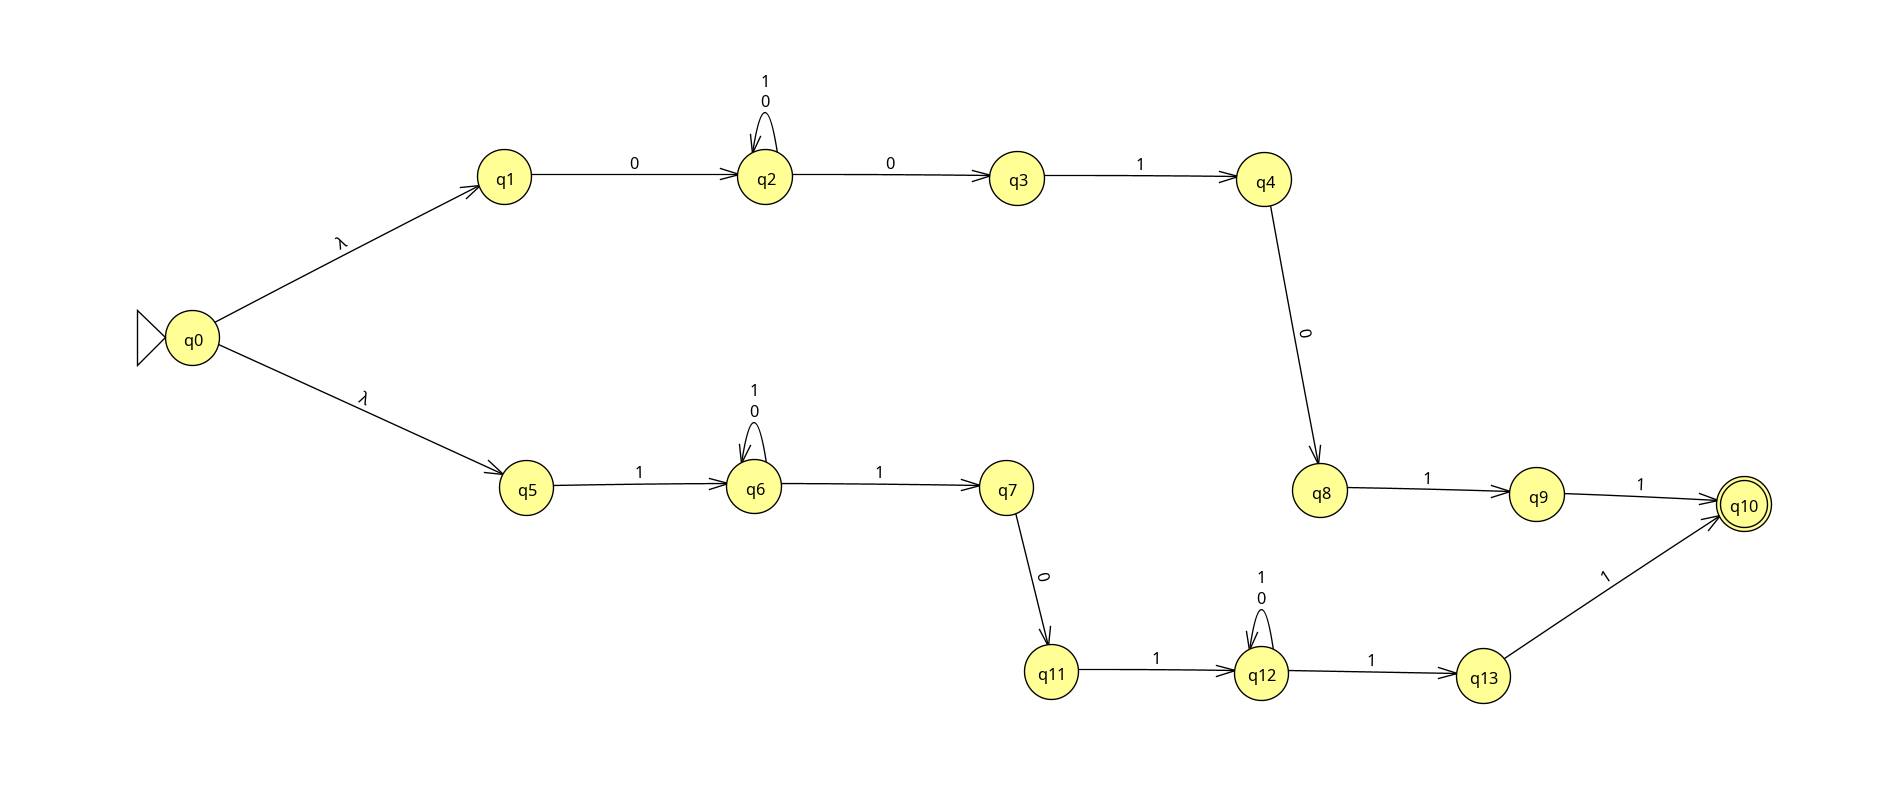
\includegraphics[width=0.85\textwidth]{img/P1/afnd_diseño.png}
    \caption{Arquitectura del AFND empleando transiciones $\lambda$ para la bifurcación semántica inicial en JFLAP.}
    \label{fig:afnd_diseno}
\end{figure}

\subsubsection{Verificación Experimental del AFND}
Todo diseño abstracto requiere validación empírica. Mediante la herramienta \textit{Multiple Run} del entorno JFLAP, se ha sometido al autómata a un riguroso banco de pruebas. Se han introducido tanto cadenas de control positivas (que cumplen íntegramente las especificaciones de sus respectivos canales) como cadenas negativas (diseñadas para fallar en el sufijo, confundir el patrón intermedio o iniciar con un bit que no corresponde a la rama evaluada).

\begin{figure}[H]
    \centering
    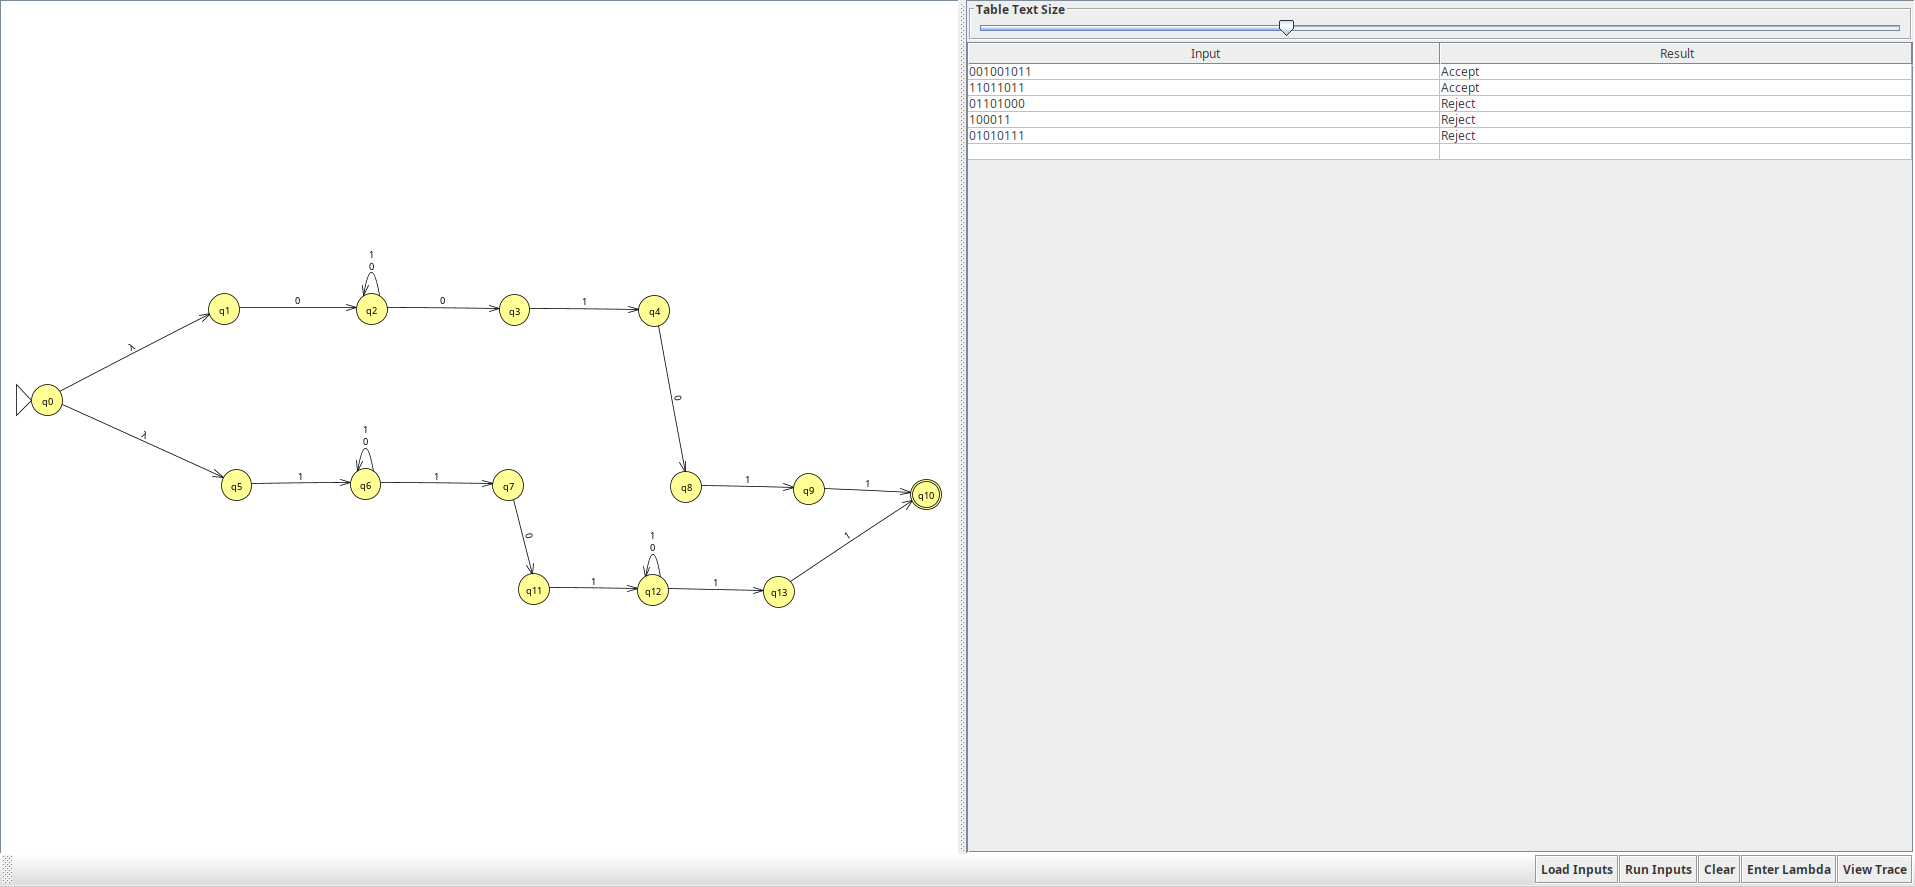
\includegraphics[width=0.85\textwidth]{img/P1/afnd_tests.png}
    \caption{Validación exhaustiva de las tramas mediante múltiples ejecuciones. Se certifica empíricamente que los rechazos y aceptaciones coinciden al 100\% con la lógica de negocio del protocolo.}
    \label{fig:afnd_tests}
\end{figure}

El análisis de las trazas de ejecución permite visualizar el comportamiento interno del algoritmo de retroceso (backtracking) de JFLAP, ilustrando cómo los hilos de procesamiento no válidos mueren al no encontrar transiciones lícitas, sobreviviendo únicamente el camino que conduce al estado de aceptación si la trama es sintácticamente correcta.

\begin{figure}[H]
    \centering
    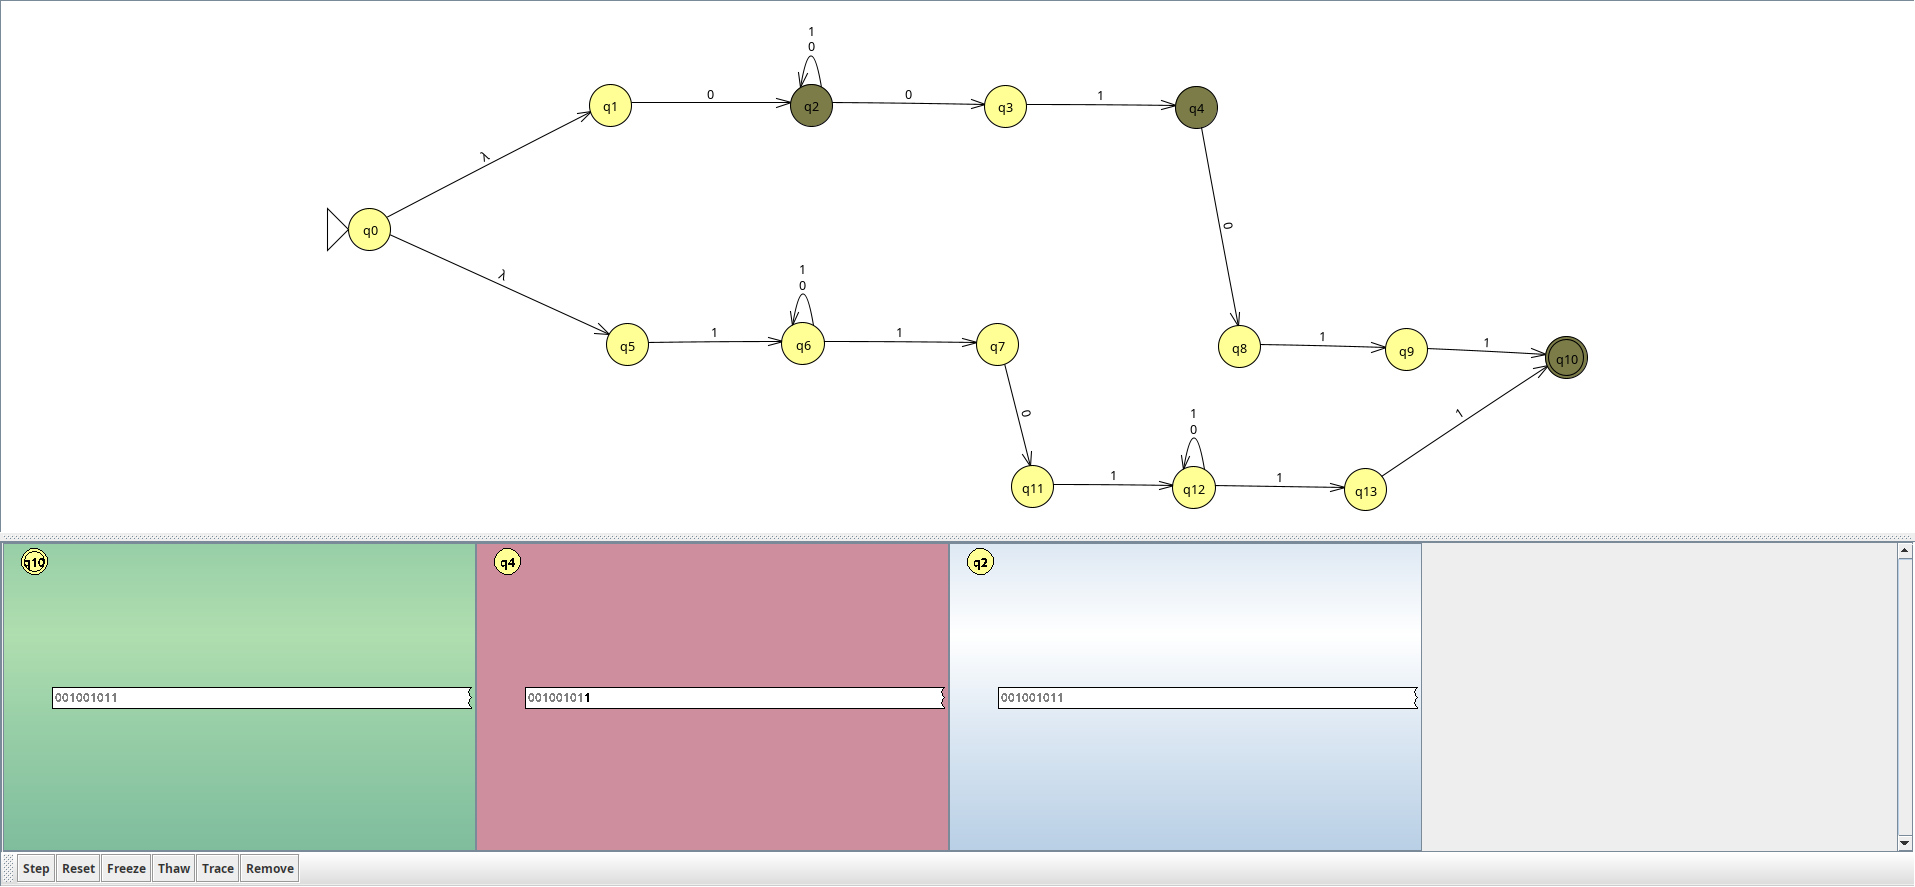
\includegraphics[width=0.85\textwidth]{img/P1/traza_1.png}
    \caption{Procesamiento de una trama válida (Traza 1) resolviendo el no determinismo.}
    \label{fig:traza_1}
\end{figure}

\begin{figure}[H]
    \centering
    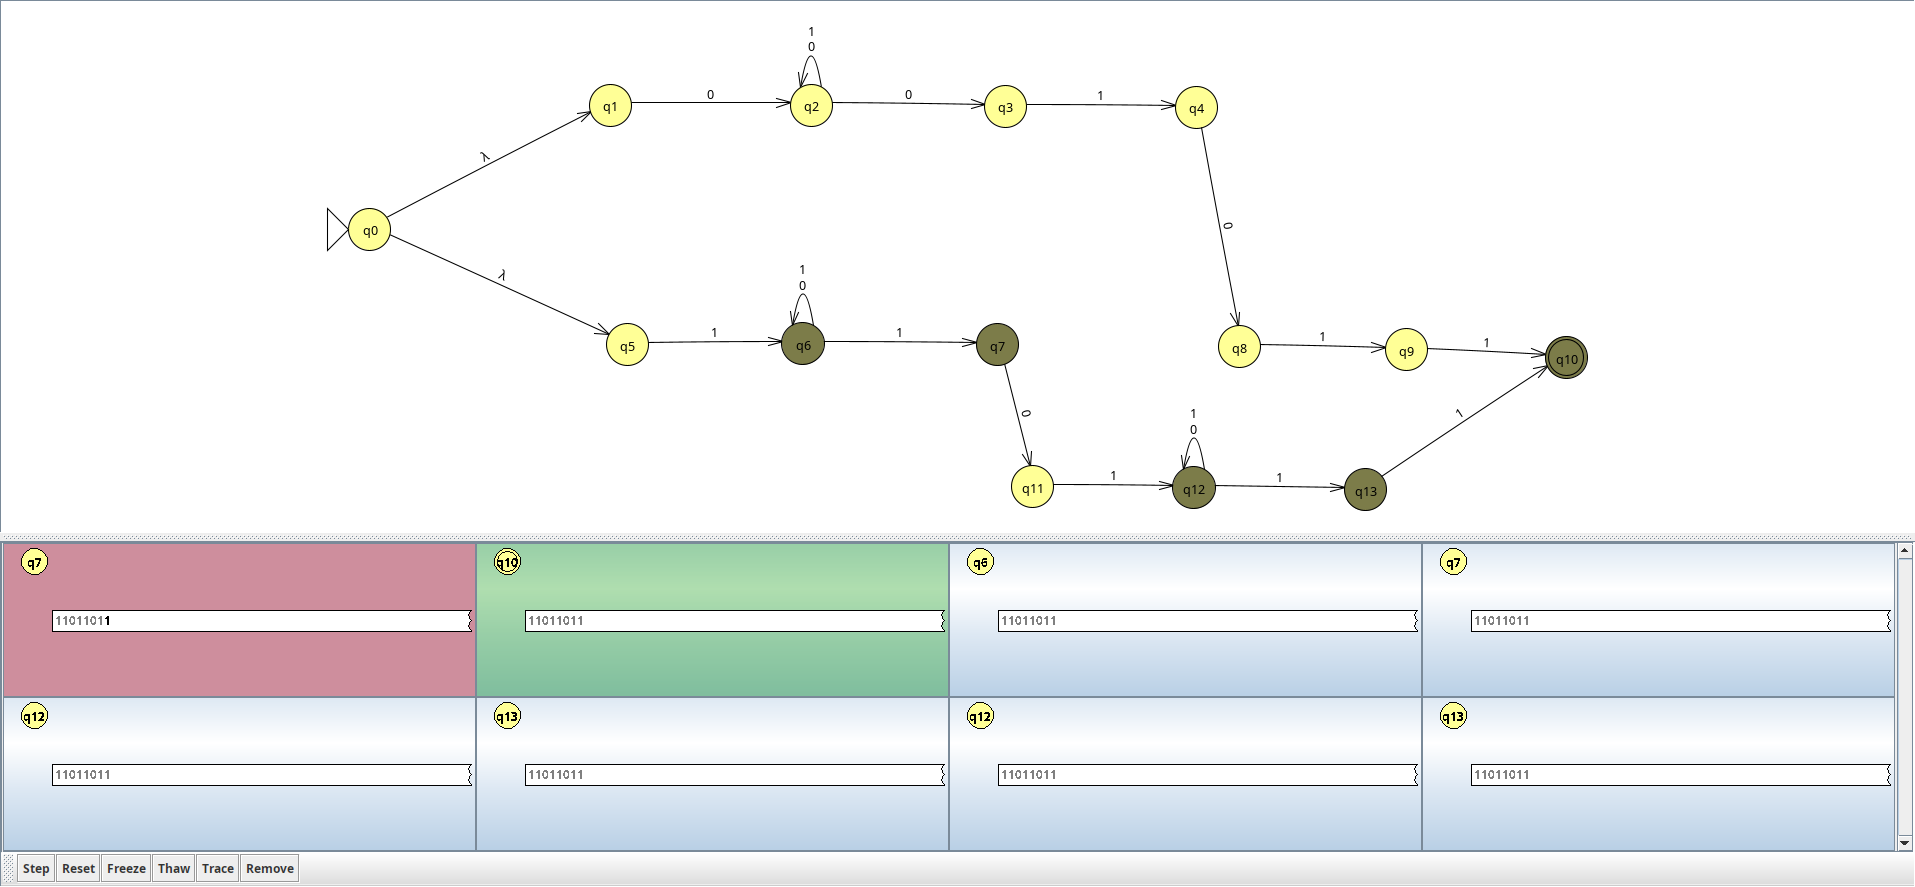
\includegraphics[width=0.85\textwidth]{img/P1/traza_2.png}
    \caption{Procesamiento de una trama válida (Traza 2) resolviendo el no determinismo.}
    \label{fig:traza_2}
\end{figure}

\subsection{Determinización del Autómata (Transformación a AFD)}
Si bien el AFND resulta idóneo para la especificación formal del problema, su implementación directa en el microcontrolador de un dispositivo periférico es computacionalmente inviable. El hardware físico opera secuencialmente y no puede asumir la sobrecarga computacional que supone evaluar caminos de forma concurrente o realizar conjeturas sobre transiciones nulas. Se requiere, por tanto, un Autómata Finito Determinista (AFD).

Para solventar esta brecha entre abstracción y hardware, se ha aplicado el \textbf{Algoritmo de Construcción de Subconjuntos} (también conocido como algoritmo de Rabin-Scott). Mediante la función \textit{Convert to Deterministic Automaton} de JFLAP, se ha calculado el cierre-$\lambda$ de todos los estados originales. Cada nuevo estado en el AFD representa un macro-estado equivalente a un conjunto de estados del AFND original. El resultado es un autómata donde, ante un estado determinado y la lectura de un símbolo concreto, solo existe una única transición posible.

\begin{figure}[H]
    \begin{center}
        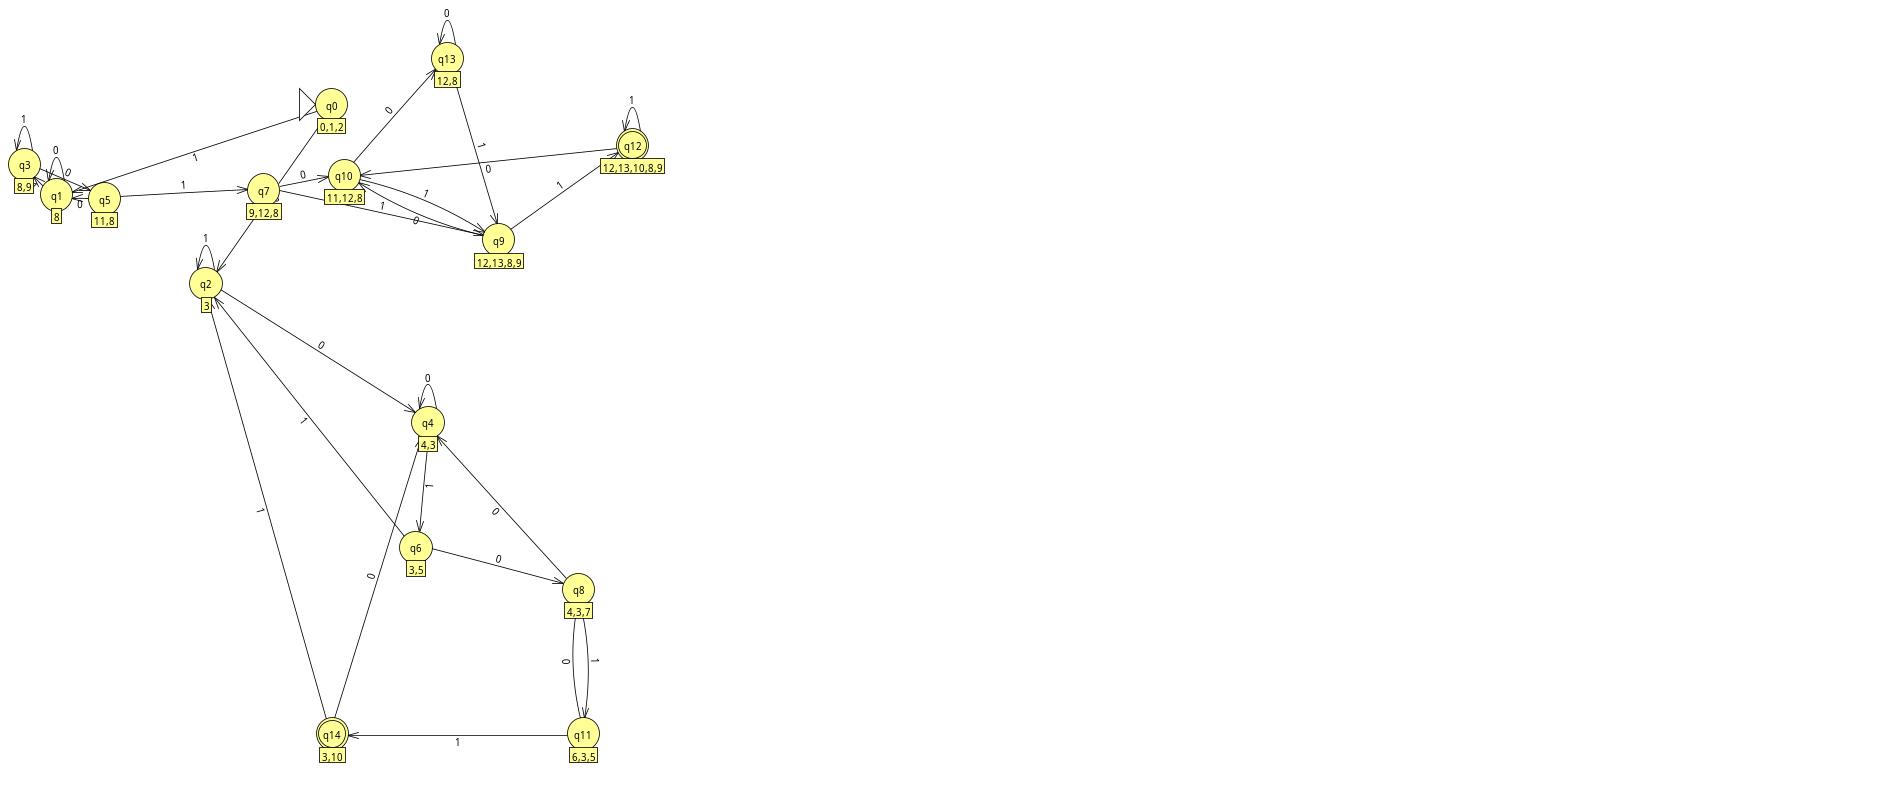
\includegraphics[width=\textwidth]{img/P1/afd_convertido.png}
    \end{center}
    \caption{Autómata Finito Determinista (AFD) resultante de la conversión. La topología refleja un incremento de la complejidad para eliminar ambigüedades.}
    \label{fig:afd_convertido}
\end{figure}

\subsection{Optimización mediante Minimización}
El algoritmo de subconjuntos garantiza el determinismo, pero a menudo produce autómatas sobredimensionados que contienen estados redundantes o inaccesibles desde el estado inicial. En el diseño de redes, minimizar la matriz de transiciones es imperativo para reducir el uso de memoria caché y optimizar los ciclos de CPU durante el análisis de paquetes.

Para lograrlo, se ha recurrido al algoritmo de partición (basado en clases de equivalencia). JFLAP, mediante su herramienta \textit{Minimize DFA}, separa iterativamente los estados finales de los no finales y continúa subdividiendo estos conjuntos basándose en el comportamiento de las transiciones. Si dos o más estados derivan en las mismas respuestas ante el mismo conjunto de entradas futuras, se consideran indistinguibles y se fusionan en un único estado lógico.

\begin{figure}[H]
    \begin{center}
        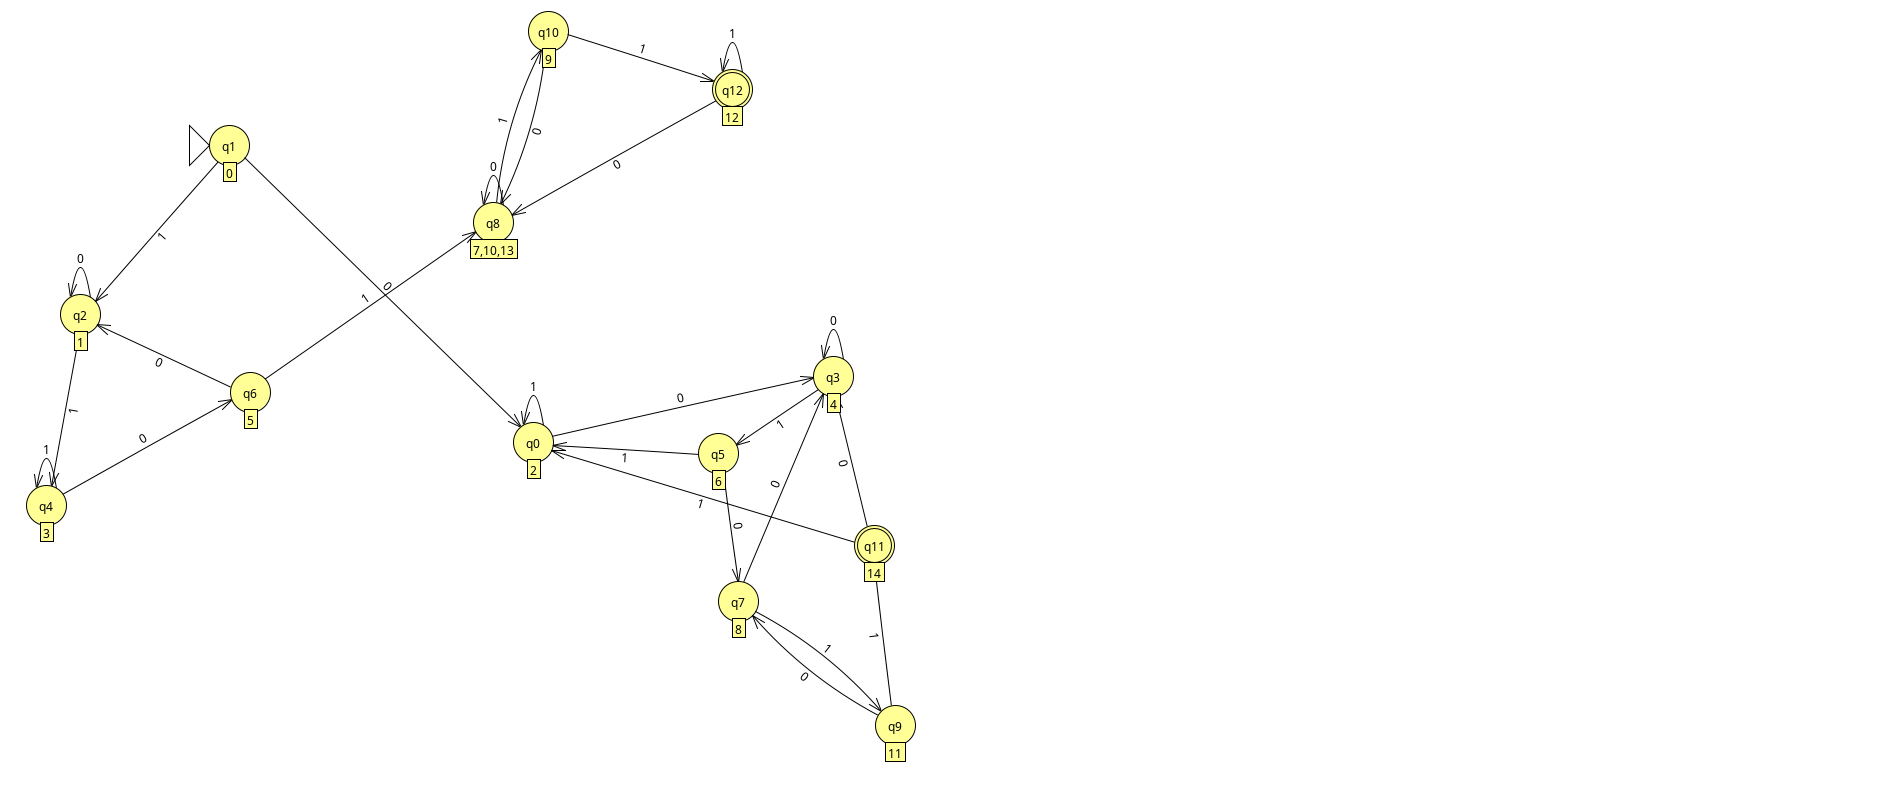
\includegraphics[width=\textwidth]{img/P1/afd_minimo.png}
    \end{center}
    \caption{Autómata Finito Determinista Minimal. Constituye la implementación de hardware de menor coste sin alterar la capacidad de reconocimiento del lenguaje.}
    \label{fig:afd_minimo}
\end{figure}

\subsubsection{Validación de Equivalencia del Autómata Mínimo}
Para ratificar matemáticamente que los procesos de determinización y minimización no han introducido derivas semánticas ni han alterado el lenguaje $L$ reconocido por el autómata original, se ha sometido al nuevo AFD minimal al escrutinio del banco de pruebas inicial. 

\begin{figure}[H]
    \centering
    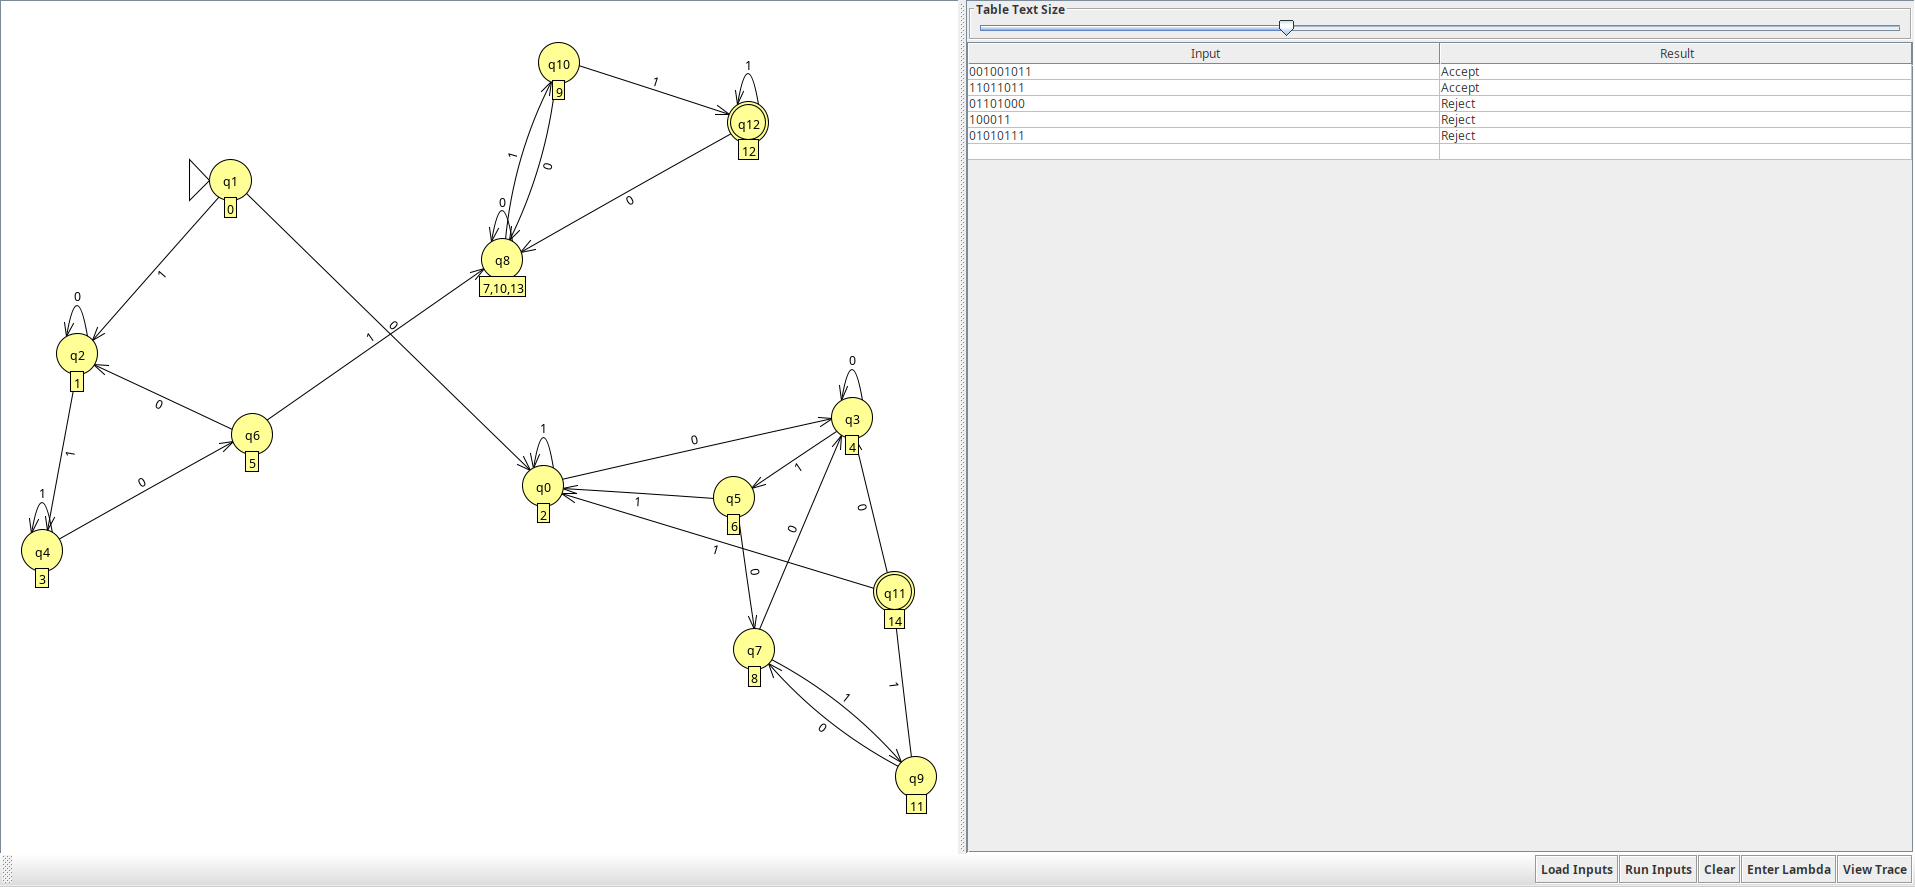
\includegraphics[width=0.85\textwidth]{img/P1/afd_minimo_tests.png}
    \caption{Re-evaluación del banco de pruebas. El comportamiento de filtrado demuestra ser absolutamente idéntico al modelo original.}
    \label{fig:afd_minimo_tests}
\end{figure}

Las trazas adjuntas a continuación corroboran que el recorrido sobre la nueva topología minimal es completamente lineal. El autómata consume un símbolo por cada transición de manera estricta y predecible, descartando paquetes erróneos inmediatamente y validando los legítimos con la máxima eficiencia.

\begin{figure}[H]
    \centering
    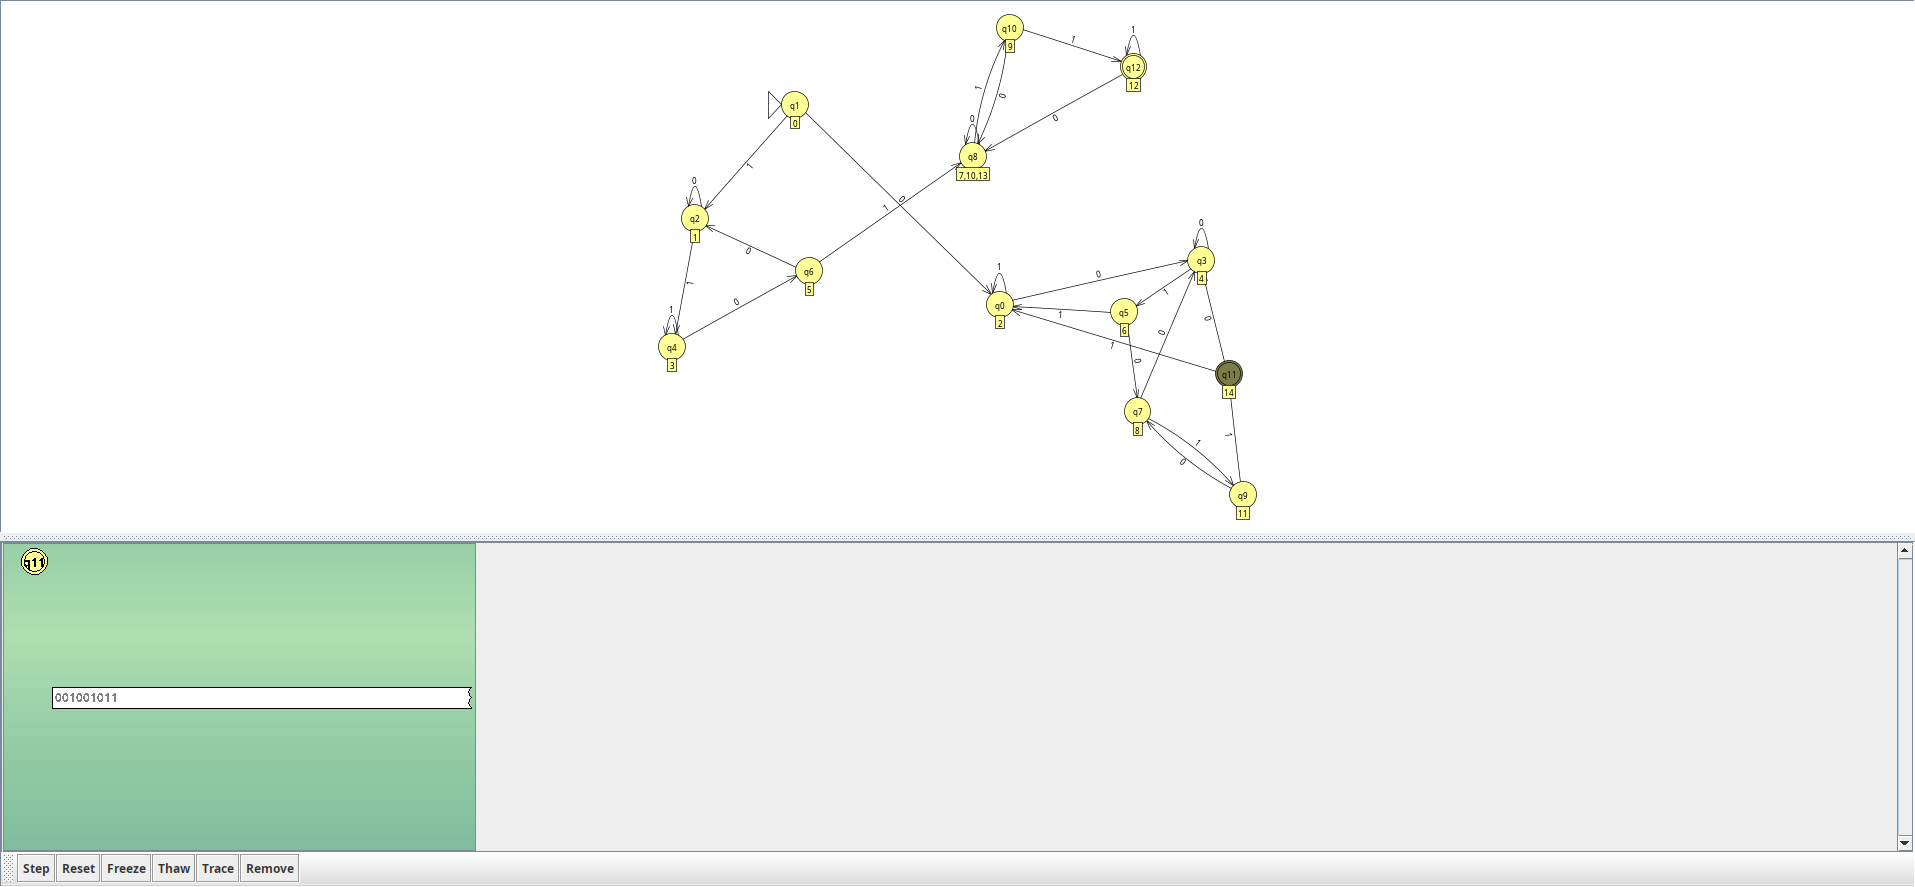
\includegraphics[width=0.85\textwidth]{img/P1/afd_minimo_trace_1.png}
    \caption{Lectura determinista e instantánea de una trama válida (Traza 1) en la versión minimal.}
    \label{fig:afd_minimo_trace_1}
\end{figure}

\begin{figure}[H]
    \centering
    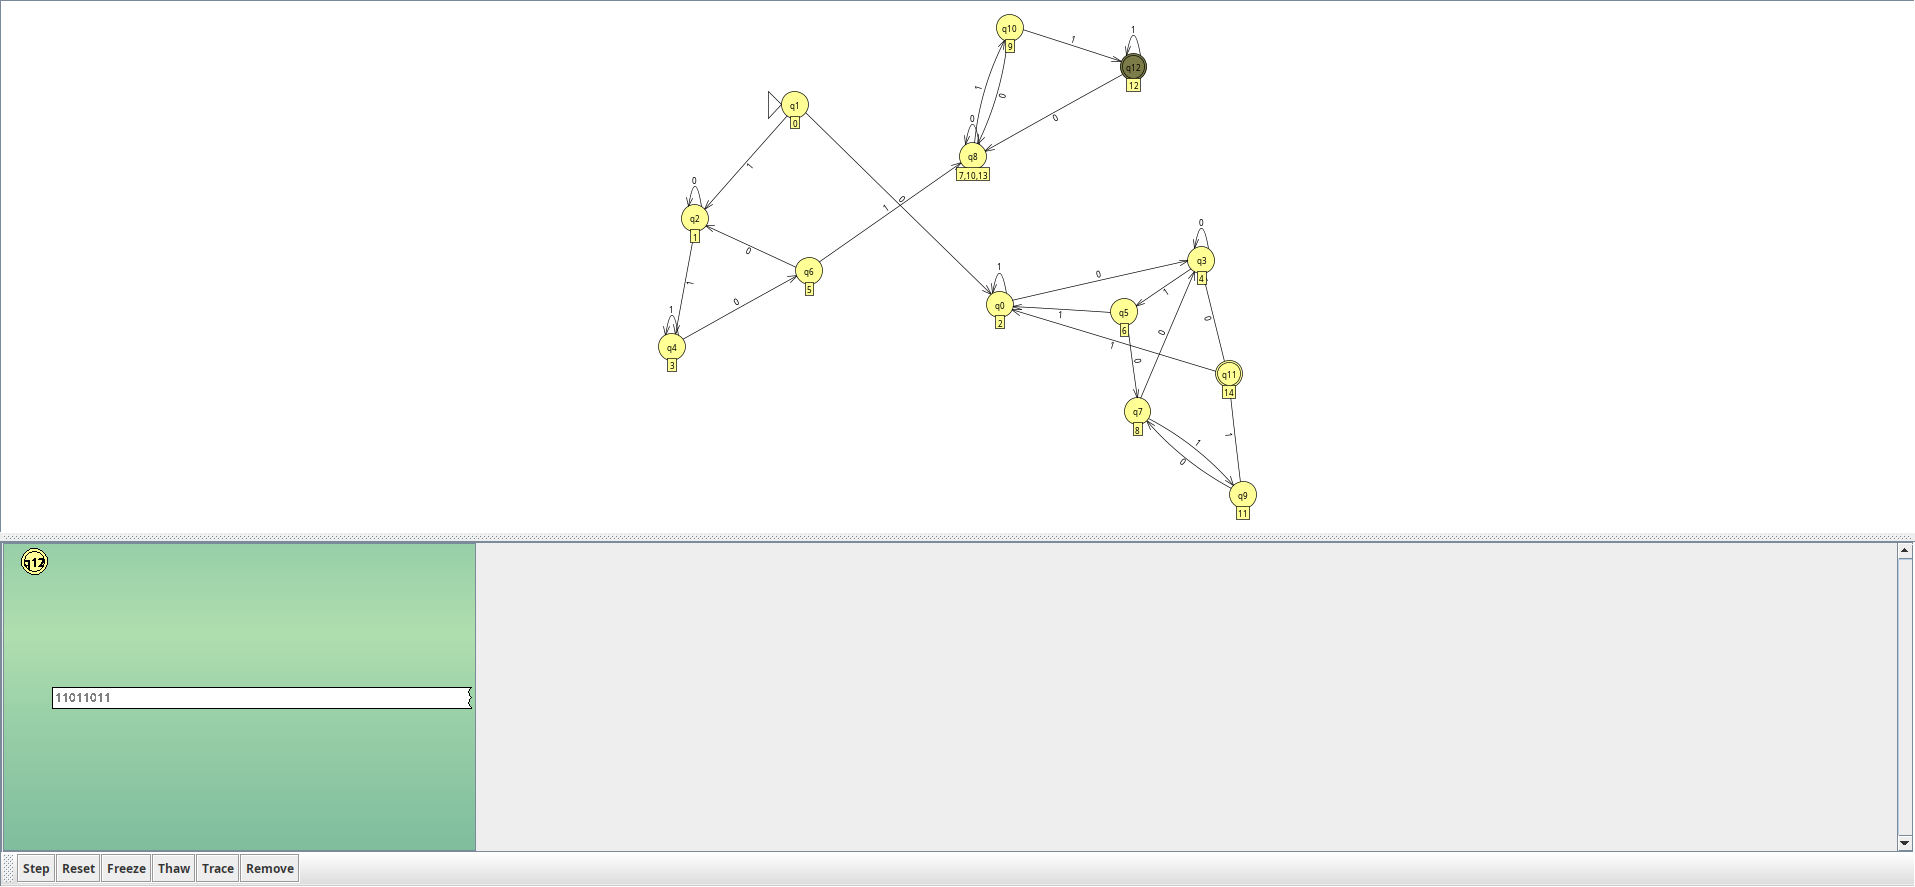
\includegraphics[width=0.85\textwidth]{img/P1/afd_minimo_trace_2.png}
    \caption{Lectura determinista e instantánea de una trama válida (Traza 2) en la versión minimal.}
    \label{fig:afd_minimo_trace_2}
\end{figure}

\subsection{Conclusiones Finales}
El desarrollo de esta práctica demuestra la potencia y necesidad de los Modelos de Computación aplicados a la Ingeniería de Software y las Comunicaciones. Se ha completado el ciclo integral del diseño lógico:
\begin{enumerate}
    \item \textbf{Definición y Abstracción:} Partiendo de un requerimiento técnico real (telemetría de doble canal IoT), se parametrizó un lenguaje regular sujeto a estrictas validaciones de prefijo, subsecuencia y sufijo (\texttt{011}).
    \item \textbf{Modelado No Determinista:} Se diseñó un AFND apoyado en transiciones nulas para simplificar el despliegue paralelo de las reglas condicionales, confirmando su validez funcional mediante \textit{tests} automatizados.
    \item \textbf{Adaptación Tecnológica y Reducción:} Mediante procesos puramente algebraicos sustentados por el software JFLAP, el modelo fue determinizado y optimizado a su mínima expresión.
\end{enumerate}
En conclusión, el autómata final obtenido no solo reconoce de manera exacta el protocolo original, sino que presenta la forma canónica ideal para ser compilado en analizadores léxicos, expresiones regulares de firewall o grabado directamente en la lógica cableada (FPGAs) de dispositivos de red.

\end{document}
